\documentclass[12pt,a4paper]{jsarticle}
\usepackage[dvipdfmx]{graphicx}
\usepackage[dvipdfmx]{color}
\usepackage{listings}
% to use japanese correctly, install jlistings.
\lstset{
  basicstyle={\small\ttfamily},
  identifierstyle={\small},
  commentstyle={\small\itshape\color{red}},
  keywordstyle={\small\bfseries\color{cyan}},
  ndkeywordstyle={\small},
  stringstyle={\small\color{blue}},
  frame={tb},
  breaklines=true,
  numbers=left,
  numberstyle={\scriptsize},
  stepnumber=1,
  numbersep=1zw,
  xrightmargin=0zw,
  xleftmargin=3zw,
  lineskip=-0.5ex
}
\lstdefinestyle{customCsh}{
  language={csh},
  numbers=none,
}
\lstdefinestyle{customRuby}{
  language={ruby},
  numbers=left,
}
\lstdefinestyle{customTex}{
  language={tex},
  numbers=none,
}
\lstdefinestyle{customJava}{
  language={java},
  numbers=left,
}
\begin{document}
\title{卒業論文\\
\vspace{4cm} hikiutilsを用いた\\卒業論文作成}
\author{ 関西学院大学 理工学部 情報科学科\\\\1234 西谷滋人}
\date{\vspace{3cm} 2017年  3月\\
\vspace{3cm} 指導教員  西谷 滋人 教授}
\maketitle
\tableofcontents

\title{hikiutilsを用いた卒業論文作成}
\author{にしたに}
\date{関西学院}
\maketitle

\section{イントロダクション}
卒業論文は,大学で課される普通の授業のレポートに比べて深い内容が要求されます.また,研究という側面から体裁や版権など出版における多くの掟を遵守しながら,高い品質を保つ必要です.そのため,指導教官との編集作業が重要となります.編集作業の効率を高めるためには,共同作業を促進するプラットフォームが必要です.

体裁などを考えるとLatexの使用が標準ですが,執筆段階での煩わしさを低減するため,Mark Up記法による文章作成が一般的です(「ドキュメント作成システム構築ガイド,GitHub, RedPen, Asciidoctor, CIによるモダンライティング」, 伊藤敬彦,吉村孝広,技術評論社).西谷研ではMark Up記法の一種であるhiki記法を用いて執筆します.hiki記法からhtmlへ変換するソフトhikidocによる容易な変換が可能なため,日記web appliのhiki diaryでも利用されている有名なソフトです.hiki記法をベースにして,wiki wiki webと同等の機能を提供するhikiシステムがgithubに公開されており,個人の手持ちのパソコンにインストールしてwikiを利用することができます.西谷研ではさらにhiki記法を拡張して,コードのカラー表示,数式のlatex記述が可能となるシステムを利用しています.

本資料では,卒論の編集作業を効率化する図に示すようなシステムの使い方を紹介します.

\begin{figure}[htbp]\begin{center}
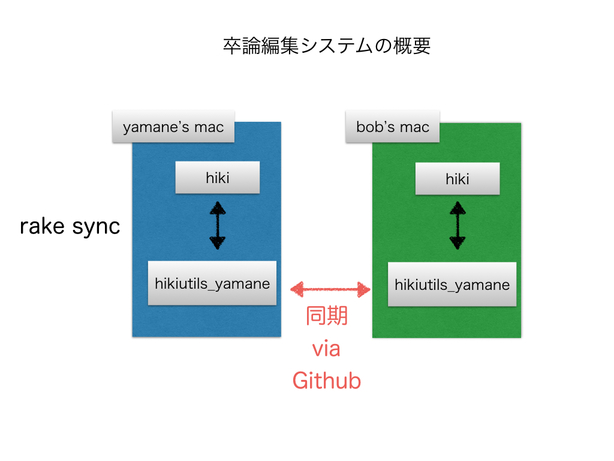
\includegraphics[width=10cm,bb= 0 0 737 453]{../figs/./hikiutils_bob.002.jpeg}
\caption{卒論編集システムの基本概念.}
\label{default}\end{center}\end{figure}
例えば,卒業生をyamaneとしましょう.yamaneの個人のMacの自分のdirectory(hikiutils\_yamane)に幾つかのファイルを作成して卒論を書いているとします.これを指導教官(bob)が編集するとします.この同期には,Githubにより提供される共同作業環境を使います.これだけでは編集中の文書の体裁がわかりにくいでしょう.そこで,hikiシステムにより容易にwebブラウザ上に完成形を表示しつつ執筆することが求められます.このような環境を提供するのが,本システムです.

\section{hikiとの同期}
\subsection{hikiutilsのinstall}
hikiuitlsをgemからinstallしておく必要がある.コマンドは以下の通り.
\begin{quote}\begin{verbatim}
gem install hikiutils
\end{verbatim}\end{quote}
さらに
\begin{quote}\begin{verbatim}
hiki -v
\end{verbatim}\end{quote}
で0.2.3.2以上であることを確認.

\subsection{個別ディレクトリーの構成}
図にhikiutils\_bobのディレクトリー構成を示す.

\begin{figure}[htbp]\begin{center}
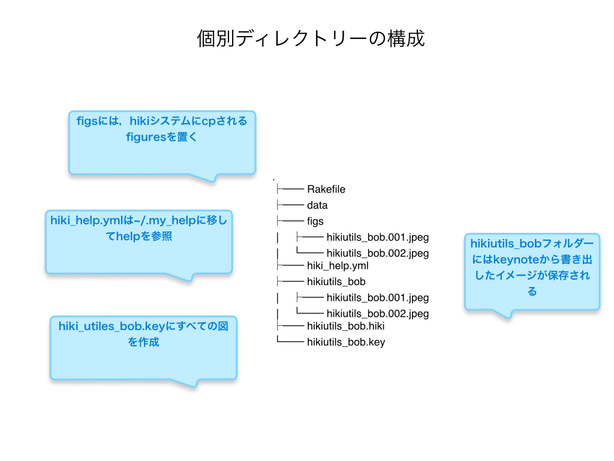
\includegraphics[width=10cm,bb= 0 0 737 453]{../figs/./hikiutils_bob.003.jpeg}
\caption{hikiutils\_bobのディレクトリー構成.}
\label{default}\end{center}\end{figure}
コマンド
\begin{quote}\begin{verbatim}
hiki -i
\end{verbatim}\end{quote}
によって以下のようなファイルが作成される.
\begin{lstlisting}[style=customCsh,basicstyle={\scriptsize\ttfamily}]
bob% ls -lat
total 1072
-rw-r--r--   1 bob  501      99  1 20 12:44 .hikirc
drwxr-xr-x   5 bob  501     170  1 20 12:44 figs/
drwxr-xr-x  12 bob  501     408  1 20 12:34 ./
-rw-r--r--   1 bob  501       8  1 20 11:01 .gitignore
-rw-r--r--   1 bob  501    3507  1 20 11:01 Rakefile
drwxr-xr-x   2 bob  501      68  1 20 11:01 data/
-rw-r--r--   1 bob  501    2595  1 20 11:01 hiki_help.yml
drwxr-xr-x  26 bob  501     884  1 20 11:00 ../
\end{lstlisting}
この.hikircにデータが設定データが自動的に入る.さらにhikiutils\_bob.hikiおよびhikiutils\_bob.keyを作成する.これで執筆ファイルの基本構成が出来上がる.

keynoteで図を作成して,hikiutils\_bob.hikiに文章を記述していく.

\subsection{システムの概要}
図に論文作成システムの概要を示している.gemのなかに作られた例えば,hikiutils\_bobなどのdirectory内にRakefileなどを次節のコマンドを使って入れる.このdirectoryでhikiutils\_bob.hikiなどのhikiフォーマットのdocumentを作っていく.rake syncによってwebを提供するhikiのtext, attach, parserなどと同期する.一方,最終の卒業論文形態であるpdfにするためにlatex\_dir内に*.texを生成する.これは次章で解説する.

\begin{figure}[htbp]\begin{center}
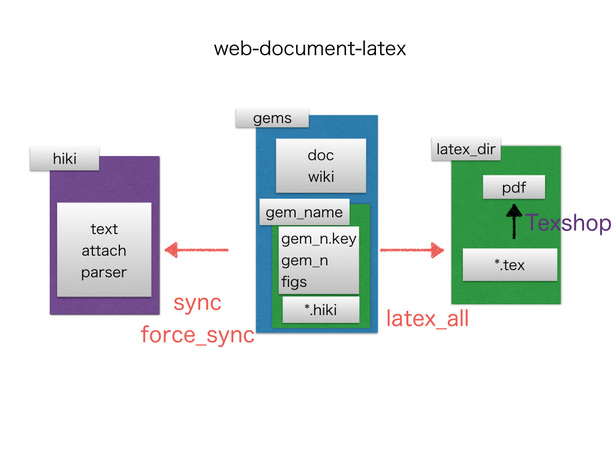
\includegraphics[width=10cm,bb= 0 0 737 453]{../figs/./hikiutils_bob.004.jpeg}
\caption{システムの概要.}
\label{default}\end{center}\end{figure}
\subsection{一般的な執筆手順}
\begin{enumerate}
\item 書類の作成
\begin{enumerate}
\item open -a mi hikiutils\_bob.hiki
\end{enumerate}
\item keynoteを開ける
\begin{enumerate}
\item open hikiutils\_bob.key
\end{enumerate}
\item keynoteのイメージをfigsに
\begin{enumerate}
\item keynoteでイメージへ書き出し(hikiutils\_bobを仮定)
\item rake convert 60 hikiutils\_bob
\end{enumerate}
\item hikiシステムとの同期
\begin{enumerate}
\item rake sync
\end{enumerate}
\item hikiシステムで表示
\begin{enumerate}
\item hiki -u hikiutils\_bob (個別のhiki fileを表示)
\item rake touch (全てを表示)
\end{enumerate}
\end{enumerate}
\subsection{rakeが用意しているタスク}
rakeの用意しているコマンドは次のとおり.
\begin{lstlisting}[style=customCsh,basicstyle={\scriptsize\ttfamily}]
rake sync             # hikiの同期
rake force_sync       # hikiの強制同期
rake chenv            # For hiki Errno::ENOENT, Errno::EACCES

rake convert          # convert fig size SCALE TARGET_DIR
rake increment        # increment fig NUBERS in FILE
rake number           # numbering figs from the NUBER in FILE

rake touch            # hikiシステムを最新状態に更新
rake github           # Githubのdirをsafariでopen
rake reset_hiki       # hikiシステムにあるゴミファイルを掃除する
\end{lstlisting}
\subsubsection{rake sync}
hikiutils\_bobにある必要な書類をhikiシステムにコピーする.その際,名前の書き換えを行う.

\begin{table}[htbp]\begin{center}
\caption{}
\begin{tabular}{lll}
\hline
hikiutils\_bobでの名前   &hikiシステムでの名前  \\ \hline
hikiutils\_bob.hiki   &hikiutils\_bob  \\
introduction.hiki   &hikiutils\_bob\_introduction  \\
\hline
\end{tabular}
\label{default}
\end{center}\end{table}
%for inserting separate lines, use \hline, \cline{2-3} etc.

figsディレクトリー内のファイルはhiki/cache/attache/hikiutils\_bobにcpされる.従って,hiki文書中で参照するには,
\verb|{{attach_view(hogehoge.png)}}|
という記述が必要となる.

\subsubsection{rake force\_sync}
hikiシステム側で直接変更を加えると,hikiutilsがsyncした時と差ができる.これを検知して,ユーザに注意を喚起する仕組みがある(rake check\_previous).これはsyncした時に自動的に呼び出される.違いの出たfilesを修正した後に強制的に同期をとるためのコマンドとして,force\_syncが用意されている.

\subsubsection{rake chenv}
hikiシステム上でerrorが出た場合(Errno::ENOENT, Errno::EACCES)に試してほしい.errorの状況は個人の設定によってちがうため,対処法の実装は網羅されていない.うまくいかない場合は西谷にIssuesとして投げるように.

\subsubsection{rake convert VAL DIR}
keynoteが吐き出したイメージを変換するためのコマンド.ImageMagickがインストールされている必要がある.ない場合は,自分でbrewからinstallするか,\verb|https://www.imagemagick.org/script/binary-releases.php|からダウンロード.うまくいかない場合はdonkeyに聞いてみてください.
\begin{quote}\begin{verbatim}
rake convert 80 hikiutils_bob
\end{verbatim}\end{quote}
によって,DIR=hikiutils\_bobにあるpngファイルをVAL=80%に縮小してfigsにためる.

\subsubsection{rake increment}
keynoteでページを追加するとhikiでの参照(attach\_view)にずれが生じる.いまのところこれを解消する方法はなく手で修正を加える必要がある.ずれが単純な場合には,
\begin{lstlisting}[style=,basicstyle={\scriptsize\ttfamily}]
cp hikiutils_bob.hiki tmp.hiki
rake increment 2 tmp.hiki > tmp2.hiki
\end{lstlisting}
としてattach\_viewのページ番号を単純に増加させることができる.

\subsubsection{rake number}
rake incrementと同じくfigs内の通し番号が変わった時にattach\_viewの通し番号を調整するコマンド.
\begin{lstlisting}[style=customCsh,basicstyle={\scriptsize\ttfamily}]
rake number 3 hikiutils_bob.hiki > tmp.hiki
cp tmp.hiki hikiutils_bob.hiki
\end{lstlisting}
とすると
\begin{lstlisting}[style=customCsh,basicstyle={\scriptsize\ttfamily}]
8c8
{{attach_view(hikiutils_bob.002.jpeg)}}
---
{{attach_view(hikiutils_bob.003.jpeg)}}
21c21
{{attach_view(hikiutils_bob.003.jpeg)}}
---
{{attach_view(hikiutils_bob.004.jpeg)}}
\end{lstlisting}
などと番号を3から順に振り替えてくれる.

\subsubsection{rake touch}
hiki touchをおこなって最新版に更新します.

\subsubsection{rake github}
git remoteにあるoriginのgithubをsafariでopenします.

\subsubsection{rake reset\_hiki}
hikiシステムにあるゴミファイルを掃除します.
\begin{lstlisting}[style=customCsh,basicstyle={\scriptsize\ttfamily}]
bob% rake reset_hiki
hikiutils: provide utilities for helping hiki editing.
"open -a mi"
target_dir : /Users/bob/Sites/nishitani0/Internal/data/text
-rw-rw-rw-  1 bob  staff    182  2  5 12:03 hikiutils_bob
-rw-rw-rw-  1 bob  staff   7220  2  5 12:03 hikiutils_bob_latex_all
-rw-rw-rw-  1 bob  staff  10104  2  5 12:03 hikiutils_bob_sync
-rw-r--r--  1 bob  staff    944  2  5 12:03 hikiutils_bob_toc
remove hikiutils_bob_toc[ynql]?
\end{lstlisting}
となります.yes, no, quit, listのなかから選んでください.

\subsection{githubによる同期}
これらの作業の流れを示すシーケンス図は次の通りである.

\begin{figure}[htbp]\begin{center}
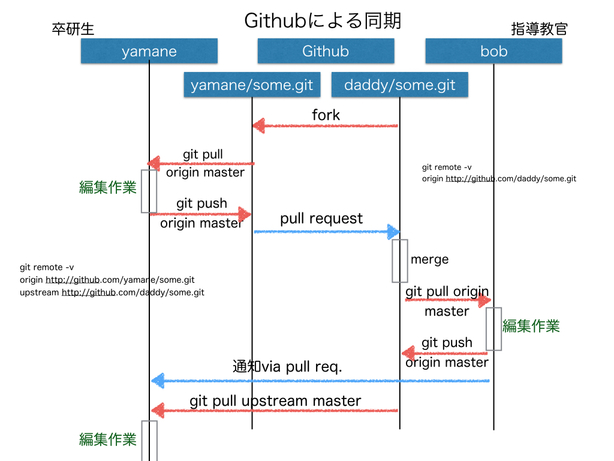
\includegraphics[width=10cm,bb= 0 0 737 453]{../figs/./hikiutils_bob.005.jpeg}
\caption{卒論編集時のgithubによる同期のシーケンス図.}
\label{default}\end{center}\end{figure}
git init, forkが済んでいると仮定して同期の手順を以下に示す.

\begin{enumerate}
\item git push作業
\begin{enumerate}
\item git add -A
\item git commit -m 'first commit'
\item git push origin master
\end{enumerate}
\item githubでbobへpull requestをかける
\item bobの編集後,通知がくる.まつことなく作業してもok.
\item git pull作業
\begin{enumerate}
\item git pull upstream master
\end{enumerate}
\end{enumerate}
以下には関連するコマンドと動作を記した.
\begin{description}
\item[git remote -v]  githubのremoteアドレスを表示

\item[git remote add upstream git@...] githubのアドレスをupstreamとして登録.

\end{description}
\subsection{hikiutil関連のヘルプ}
\subsubsection{hikiで卒論を書くときの初期化と掟}
\begin{itemize}
\item 目的:西谷が後で迷わないように決まったファイル構造を堅持すべし
\item 文書:hikiで書く.のちには,latexに変換するプログラムを提供します
\item 図表:すべての図表をkeynoteにまとめる,タイトルを分かりやすく書く
\item データ:dataディレクトリにまとめる.ファイル名をkeynoteの対応する図表中に記す
\item hiki --initializeで初期ファイル(Rakefile, ./.hikirc, hiki\_help.yml)がcopyされる
\item hiki\_help.ymlを適宜~/.my\_helpにcopyしてhiki\_helpとして利用,(my\_help参照)
\item Errno::EACCESやpermission errorがでたときはrake chenvを試してみる(報告して)
\item rake syncによってhikiディレクトリーと同期が取られる
\item hiki -u TARGETによってブラウザー表示される
\item テキストの拡張子は'.hiki'
\item hikiでのurlはテキスト前とディレクトリーから自動生成される
\item 例えば,hiki2latex\_saki/introduciton.hikiとするとhiki2latex\_saki\_introducitonと変換される
\end{itemize}
\subsubsection{図表に関する制約}
\begin{itemize}
\item すべての図表をkeynoteにまとめる
\item keynoteに書いたスライドはイメージに書き出して,rake convert 80 TARGET\_DIRでfigsに変換
\item rake syncでfigsにあるfilesはhiki/target\_dirにcpされる
\item \verb|convert #{source} -resize 20% #{target}によって,target=figs/TAERGET.pngに20%に縮小して保存される|
\item convert -density 300 view.svg view.pngで300dpiで変換
\item attach\_anchorでは'\verb|{{attach_anchor(test.png, hiki2latex_saki)}}|'と,directory指定しなければならない.
\item keynoteであとで図を挿入して番号が変わった時の原稿の一括変換
\item rake increment 2 boundary\_bob.hiki boundary\_bob > tmp.hiki
\item rake convert 60 boundary\_bob
\item rake sync
\item hiki -u boundary\_bob\_tmp
\end{itemize}
\subsubsection{同期に関する制約}
\begin{itemize}
\item hikiはフラットなdirectory構造を取っている
\item hikiの文書はスネーク表記(例えば,latex2hiki\_saki)で階層構造に似せている
\item hikiのurlの接頭語となる名前をbasenameのdirectory名とする.
\item directory名が'hikis'である場合はその親directory名となる.
\item ~/.hikircのtarget directoryを同期先のdirectoryとする.
\item ~/.hikircがない場合は同期先のdirectoryを聞く.
\item それらは./.hikircに保存される
\end{itemize}
\subsubsection{テキストに関する制約}
\begin{itemize}
\item テキストの拡張子は'.hiki'としている
\item hikiでのurlはテキスト前とディレクトリーから自動生成される
\item 例えば,hiki2latex\_saki/introduciton.hikiとするとhiki2latex\_saki\_introducitonと変換される
\end{itemize}


\section{実際の最終形態(卒論=pdf)への変換}
hiki+keynoteで卒論の内容ができたら,それを卒論の最終形態つまりpdfへ変換する必要が出てきます.

ここで問題が発生します.hikiよりもlatexの方が機能が豊富なこと.
つまり,簡易に書くにはhikiなどのmark downで書いていくのがいいんですが,
文書として完成度を高めるには,latexで細かい設定を調整する必要がどうしても出てきます.

具体的には,

\begin{enumerate}
\item 図の配置を調整するwrapの数値調整
\item 図のcaptionとlabel-ref(hikiutilsで対応)
\item 参照文献referenceとcite-bibitem(hikiutilsで対応)
\item リスト,引用の体裁(hikiutilsで対応)
\item 章立て階層構造(hikiutilsで対応)
\end{enumerate}
などが問題になるところです.ほとんどをhikiutilsで提供していますが,
いざという時の微調整は必要です.

これはhikiではどうしようもありません.一つの手はもう少し高機能なmark up言語
例えばasciidocなどに変更することですが,これはどこまでいっても終わりのない
方向のようで,結局はlatexで書いているのと同じになる可能性があります.

我々は違う戦略をとります.それは,
\begin{quote}\begin{verbatim}
latexをベースにして,hikiを生成する
\end{verbatim}\end{quote}
と言う手です.

DRY(Don't Repeat Yourself)原則さえ守れば,文書管理はいいのですから,
ある段階まですすめばhikiではなくlatexを原本にするのです.
そのための変換器latex2hikiとその派生rake環境が用意されています.
そちらはこちらで卒業後に変換します.参照文献はlatexに移してから
修正してください.

ここでは,hikiでできることをとことん突き詰めておきます.

\subsection{install}\begin{quote}\begin{verbatim}
hiki -i
\end{verbatim}\end{quote}
でinstallされています.新たに使うコマンド群は次の通りです.
\begin{quote}\begin{verbatim}
rake latex            # FILE1をlatexに変換
rake latex_all        # すべてのhikiファイルをlatex変換
rake latex_wrap       # FILE1をwrap formatでlatexに変換
rake reset_latex_dir  # latex_dirのゴミファイルを削除
\end{verbatim}\end{quote}
\subsection{rake latex(個別ファイルの変換)}\begin{quote}\begin{verbatim}
rake latex sync.hiki
\end{verbatim}\end{quote}
とすると,
\begin{quote}\begin{verbatim}
latex_dir/sync.tex
\end{verbatim}\end{quote}
にlatex変換後のファイルが生成します.これを,TeXShopでcommand\_t変換します.
完成例はこちらです.

\begin{itemize}
\item \verb|{{attach_anchor(sync.pdf,hikiutils_bob)}}|
\end{itemize}
うまくいかないときは,terminalで
\begin{quote}\begin{verbatim}
platex sync.tex
dvipdfmx sync.dvi
\end{verbatim}\end{quote}
を試してみてください.

\subsubsection{注意}
hikiの初めの部分は,
\begin{lstlisting}[style=customCsh,basicstyle={\scriptsize\ttfamily}]
bob% head -3 hikiutils_bob.hiki
! title:hikiutils -iによる卒論作成システム
! autor:Shigeto R. Nishitani
! date: Kwansei Gakuen Univ., 2017/1
\end{lstlisting}
とすると,
\begin{lstlisting}[style=customTeX,basicstyle={\scriptsize\ttfamily}]
\begin{document}
\title{hikiutils -iによる卒論作成システム}
\author{Shigeto R. Nishitani}
\date{ Kwansei Gakuen Univ., 2017/1}
\maketitle
\end{lstlisting}
と変換してくれます.次節のlatex\_allでは,basename.hikiに書かれたそれらの情報は,
head.texでtitleなどを用意するべきなので,自動で消されます.

必要な図は,figsから自動で取るようになっていますが,
サイズや解像度が問題のときは手動で調整してください.

\subsection{rake latex\_all手順(ディレクトリー内の一括変換)}
pwdのdirectoryと同名のbasenameに.hikiの拡張子がついたファイルが用意されていて,
\begin{quote}\begin{verbatim}
rake latex_all
\end{verbatim}\end{quote}
をおこなうと自動で全部を一体にまとめた文書へのlatex変換が出来上がります.
たとえば,hikiutils\_bob.hikiの記述を
\begin{lstlisting}[style=customCsh,basicstyle={\scriptsize\ttfamily}]
bob% cat hikiutils_bob.hiki 
!hikiutilsを用いた卒業論文作成

! [[hikiutils_bob_sync]]
! [[hikiutils_bob_latex_all]]

\end{lstlisting}
とすると,sync.tex, latex\_all.texがlatex\_dir内に変換されます.
さらに,開いているhikiutils\_bob.texをTeXShopで変換してみてください.

うまくできないときは\verb|ここ(http://qiita.com/hideaki_polisci/items/3afd204449c6cdd995c9)|を参照して自力で入れてみてください.だめならdonkey.

\begin{itemize}
\item \verb|{{attach_anchor(hikiutils_bob.pdf,hikiutils_bob)}}|
\end{itemize}
というようになります.

\subsubsection{下準備}
latex\_dir内に幾つかのtex雛形を入れておく必要があります.
\begin{quote}\begin{verbatim}
hiki -i
\end{verbatim}\end{quote}
とhikiutils環境を再度初期化すると,自動でインストールする設定です.
なかったら手動で作ってください.Rakefile以外は上書きしません.
また,latex\_dir/head.texは下に記す修正が必要です.

\paragraph{head.tex}
題目,学生番号,氏名を変更する.年月をチェック.
\\setcounter\{tocdepth\}はtocをどこまで表示するかのレベルに対応します.
原稿作成時は階層がわかりやすいように深めにしていますが,本番では2程度で十分です.
\begin{lstlisting}[style=customTeX,basicstyle={\scriptsize\ttfamily}]
bob% cat head.tex
\title{卒業論文\\
\vspace{4cm} hikiutilsを用いた\\卒業論文作成}
\author{ 関西学院大学 理工学部 情報科学科\\\\1234 西谷滋人}
\date{\vspace{3cm} 2017年  3月\\
\vspace{3cm} 指導教員  西谷 滋人 教授}
\maketitle
\setcounter{tocdepth}{6} %

\end{lstlisting}
\paragraph{pre.tex}
latex\_allのときは使っていません.formatedの時に読むようにしていますが...読めてないようです.いずれ調べます.

\paragraph{mainのpreamble部}
あまり変更しないほうがいいですが,いずれいじることになります.
例えば,フォントポイント数を12から10ptに変えるなどです.
\begin{lstlisting}[style=customTeX,basicstyle={\scriptsize\ttfamily}]
\documentclass[12pt,a4paper]{jsarticle}
\usepackage[dvipdfmx]{graphicx}
\usepackage[dvipdfmx]{color}
\usepackage{listings,jlisting}% to use japanese correctly, install jlistings.
\lstset{
  basicstyle={\small\ttfamily},
  identifierstyle={\small},
  commentstyle={\small\itshape\color{red}},
  keywordstyle={\small\bfseries\color{cyan}},
  ndkeywordstyle={\small},
  stringstyle={\small\color{blue}},
  frame={tb},
  breaklines=true,
  numbers=left,
  numberstyle={\scriptsize},
  stepnumber=1,
  numbersep=1zw,
  xrightmargin=0zw,
  xleftmargin=3zw,
  lineskip=-0.5ex
}
\lstdefinestyle{customCsh}{
  language={csh},
  numbers=none,
}
\lstdefinestyle{customRuby}{
  language={ruby},
  numbers=left,
}
\lstdefinestyle{customTex}{
  language={tex},
  numbers=none,
}
\lstdefinestyle{customJava}{
  language={java},
  numbers=left,
}

\end{lstlisting}
\subsection{補助コマンドの解説}
\subsubsection{rake reset\_latex\_dir(latex\_dirのゴミ掃除)}
わかりやすいようにまとめたり,ファイルの名称を変更した時には,過去のtexファイルが残る.
それらを整理する時に使用.head.texだけをescapeしてrm -rfで消すので,注意が必要.
特に図形のfilesやbb filesは消えるので注意.

\subsubsection{wrap関係}
figure環境をwrapfigure環境で作るための幾つかのコマンド群です.
卒論ではfigure環境で作る方がいいんですが,journal論文などのページ数が制限された場合は,
wrapfigureでtextの回りこみや位置調整を行う必要があります.
それらのための環境を埋め込む仕組みです.

\begin{itemize}
\item rake change\_wrap(wrapで変換)
\item rake latex\_base(latexに変換するだけの下請け)
\item rake latex\_wrap(figure環境だけをwrapfig環境に変える)
\end{itemize}
Rakefile内の記述は
\begin{lstlisting}[style=customRuby,basicstyle={\scriptsize\ttfamily}]
desc "latex conversion FILE1"
task :latex => [:latex_base] do
  exit
end

desc "latex conversion FILE1 with wrap format"
task :latex_wrap => [:latex_base, :change_wrap] do
  exit
end
\end{lstlisting}
となっています.つまり,:latex\_baseをした後に,:change\_wrapを呼び出しています.

完成例はこちらです.

\begin{itemize}
\item \verb|{{attach_anchor(calphad_bob.pdf,hikiutils_bob)}}|
\end{itemize}
発表会の予稿ハンドアウトなどではこれが不可欠です.

\subsection{参照のシステム}
latexへ文献参照を渡すために,下記のようなフォーマットでの記述を行ってください.
\begin{lstlisting}[style=customCsh,basicstyle={\scriptsize\ttfamily}]
図{{ref(fig:SystemOverview)}}に卒論編集システムの概観を示しています.

!!!caption: (fig:SystemOverview)卒論編集システムの概観.
{{attach_view(hikiutils_bob.006.jpeg)}}

*基本的な使い方{{cite(listings1)}}
*独自のカラー化{{cite(listings2)}}
!reference:
:listings1:[[http://d.hatena.ne.jp/mallowlabs/20061226/1167137637]]
:listings2:[[http://www.ipc.akita-nct.ac.jp/~yamamoto/comp/latex/make_doc/source/source.html]]
\end{lstlisting}
\begin{itemize}
\item caption以下の丸括弧内にタグを書きます.
\item fig:以下のタグにsnake nameは使えません.Camelで書くようにしてください.
\item refでそれを参照します.
\item citeの方も同じです.
\item reference:以下の:...:記述がlatexではbibliographyに変わります.
\end{itemize}
これをsync, all\_latexをかけると図\ref{fig:CiteRefSystems}のようになります.latexの文献参照(cite, bibliography),図表番号の参照(ref, label)が正常に処理されていることが確認できます.また,web表示した場合でもそれほど違和感なく読めるでしょう.

\begin{figure}[htbp]\begin{center}
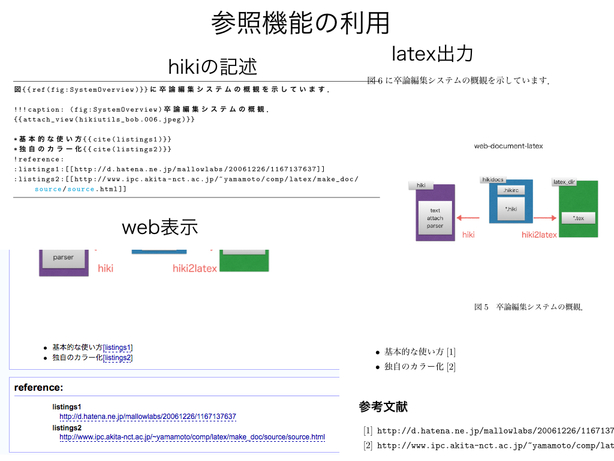
\includegraphics[width=12cm,bb= 0 0 737 553]{../figs/./hikiutils_bob.007.jpeg}
\caption{参照機能を利用した場合の変換後の表示.}
\label{fig:CiteRefSystems}
\label{default}\end{center}\end{figure}
\subsection{latexに関する制約}
\begin{itemize}
\item latex\_dirに対応するtexファイルが作られる
\item head.texにlatexのtitle部を記述
\item ref:図\ref{fig:SystemOverview}に卒論編集システムの概観を示しています.
\item !!!caption: (fig:SystemOverview)卒論編集システムの概観.
\item caption以下の丸括弧内にタグを書く
\item fig:以下のタグにsnake nameは使えん.Camelで書く
\item cite:基本的な使い方\cite{listings1}
\item !reference:
\item :listings1:\verb|http://d.hatena.ne.jp/mallowlabs/20061226/1167137637|
\item reference:以下の:...:記述がlatexではbibliographyに変わる
\end{itemize}

\end{document}
